\section{Verificação computacional reproduzível}
\label{sec:verification}

Os experimentos são determinísticos. O script \path{compilar.sh} coordena seis
programas: \path{reproduzir_curvas.py} e os cinco programas de
\path{reproducibility/selecao/}. Os arquivos JSON correspondentes registram os
testes e os valores tabulados. O arquivo
\path{reproducibility/biblioteca/resultados.json} registra também as versões
efetivamente usadas. Na execução de referência que acompanha este manuscrito:
Python 3.12.13, NumPy 2.3.5 e Matplotlib 3.10.8. A auditoria independente
também executou as seis suítes com Python 3.10.12; por isso, o requisito do
pacote é Python 3.10 ou posterior.

\subsection{Indexação}

Foram verificados:
\begin{itemize}[leftmargin=1.6em]
 \item $\pi(\pi^{-1}(n))=n$ e a ida e volta da descompactação quádrupla para $0\le n<20,000$;
 \item unicidade dos primeiros $5,000$ termos de $Q$ e $Q^{\!*}$, ausência de zero na segunda enumeração e a desigualdade de posto $j<3\height(Q(j))^2$ em ambas;
 \item $CW(2^{q-1})=1/q$ para $1\le q\le20$.
\end{itemize}
Esses testes auditam computacionalmente as identidades demonstradas.

\subsection{Conversão ReLU e minimização em catálogos finitos}

As rotinas públicas \texttt{assembly\_to\_relu} e
\texttt{relu\_to\_assembly} implementam as duas direções do
\cref{thm:assembly-relu}. Foram geradas deterministicamente $4.096$ montagens
racionais, com duas a sete folhas. Em aritmética
\texttt{fractions.\allowbreak Fraction}, o script verificou exatamente, em cada folha, os
valores nos dois extremos e no centro, a inclinação local, a largura
$N-1$ da rede e a igualdade da assinatura linear por partes após a conversão
inversa. Não há tolerância de ponto flutuante nesses testes.

O \cref{alg:finite-enumeration} foi executado sobre a raiz
$K=J_{0,0}=[0,1]$. O funcional de teste também é exato:
\begin{equation}
 \mathcal J(g)=\sum_{x\in\{0,1/4,1/2,3/4,1\}}
 \bigl(g(x)-2|x-1/2|\bigr)^2.
 \label{eq:catalog-test-objective}
\end{equation}
Cada caso foi enumerado uma segunda vez com a ordem de árvores e átomos
invertida. O conjunto de funções, a menor representação de cada função, o
valor mínimo e o fluxo vencedor permaneceram idênticos.

A \cref{tab:catalogos-pt} reúne as cardinalidades, as redundâncias de
representação e os minimizadores exatos dessas instâncias.

\begin{table}[t]
\centering
\caption{Enumeração e minimização exatas em
$\Sigma_{D,H}^{\Library}([0,1])$.}
\label{tab:catalogos-pt}
\small
\begin{tabular}{rrrrrr}
\toprule
$D$ & $H$ & representações & funções & $\min J$ & bits do desempate\\
\midrule
0 & 2 & 42 & 42 & $\frac{29}{32}$ & 12\\
1 & 2 & 102 & 96 & $0$ & 33\\
2 & 2 & 102 & 96 & $0$ & 33\\
0 & 3 & 210 & 210 & $\frac{19}{24}$ & 18\\
\bottomrule
\end{tabular}

\end{table}

A coluna ``representações'' é maior que a coluna ``funções'' quando árvores
redundantes avaliam no mesmo objeto; o desempate é feito somente depois dessa
deduplicação funcional. O salto de $D=0$ para $D=1$, $H=2$, inclui a montagem
em V que realiza exatamente o alvo de \eqref{eq:catalog-test-objective}. Já
$D=2$, $H=2$, não acrescenta folhas de escala $k=2$, pois sua altura atômica é
pelo menos $3$. O script verifica ainda as inclusões de
\eqref{eq:catalog-nesting} e a monotonicidade dos valores mínimos.

\subsection{Roundtrip dos formatos de codificação}

Os codificadores de \cref{subsec:coding-formats} e seus decodificadores foram
executados nas mesmas $4.096$ montagens racionais usadas no teste ReLU. Em
todos os casos, o fluxo atômico recuperou a assinatura linear por partes e os
dois fluxos ReLU recuperaram exatamente cada \texttt{Fraction} da rede. Foram
também verificadas, parâmetro a parâmetro, as cotas
\eqref{eq:slope-jump-height}--\eqref{eq:intercept-height}.

A fatia $N=2$ da família de \eqref{eq:coding-gap-family} permite comparar os
comprimentos sem regressão nem ajuste assintótico. A
\cref{tab:codificacoes-pt} dá os valores exatos e a
\cref{fig:codificacoes-pt} mostra as ordens de crescimento:
\begin{table}[t]
\centering
\caption{Comprimentos exatos dos três fluxos prefix-free na família crítica.}
\label{tab:codificacoes-pt}
\small
\begin{tabular}{rrrrr}
\toprule
$H$ & $L_{\rm atom}$ & $L_{\rm ReLU,str}$ & $L_{\rm ReLU,rat}$ & razão rat./str.\\
\midrule
4 & 29 & 31 & 35 & 1.129\\
8 & 33 & 35 & 51 & 1.457\\
16 & 37 & 39 & 83 & 2.128\\
32 & 41 & 43 & 147 & 3.419\\
64 & 45 & 47 & 275 & 5.851\\
128 & 49 & 51 & 531 & 10.412\\
\bottomrule
\end{tabular}

\end{table}

\begin{figure}[t]
 \centering
 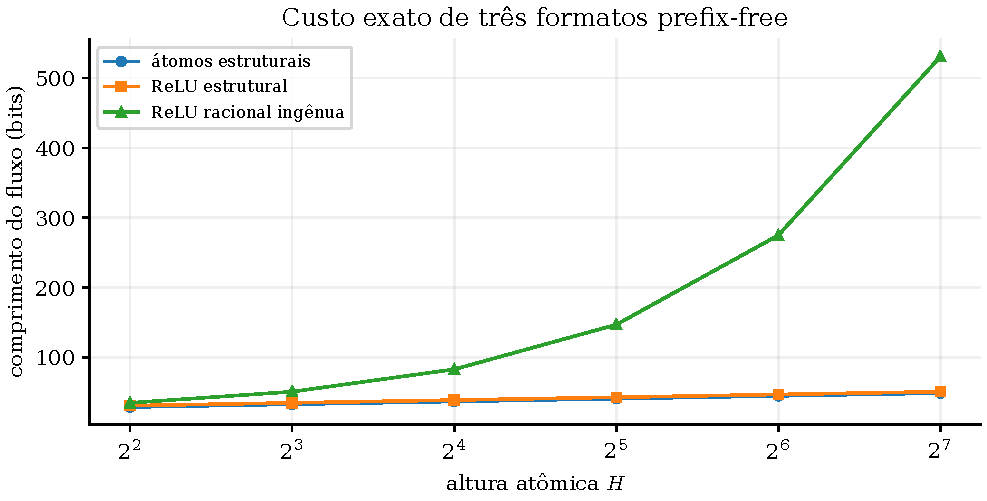
\includegraphics[width=.82\linewidth]{fig08_codificacoes.pdf}
 \caption{O par diádico estrutural mantém o custo logarítmico; expandir o
 denominador $2^k$ como parte de uma fração racional produz a sobrecarga
 linear prevista pelo \cref{thm:coding-formats}.}
 \label{fig:codificacoes-pt}
\end{figure}

\subsection{Orçamento conjunto de folhas, altura e bits}

A construção do \cref{thm:joint-budget} foi executada integralmente em
aritmética \texttt{Fraction} para $N=2,4,\ldots,256$ e quatro funções
racionais da bola $\mathcal F_{1,8}$: quadrática, constante, afim e racional
sem polo. Ao todo foram inspecionadas $2.040$ folhas. O script verificou,
sem tolerância numérica, continuidade, inclinações não nulas, erro nodal no
máximo $1/(2N^2)$, a cota $\height_{\max}\le18N^2$ e as cotas individuais
para intercepto, nós, inclinação inicial e saltos ReLU. Os três fluxos foram
decodificados de volta em cada escala.

Na sonda quadrática $f_\star(x)=4x(x-1)$, o erro uniforme foi maximizado
exatamente nos extremos e no único ponto crítico de cada folha. Isso produz
as frações da \cref{tab:joint-budget-pt}; em todas as linhas,
$N^2\|f_\star-g_N\|_\infty=49/64$, enquanto o certificado do teorema é
$3/2$ na mesma normalização (equivalentemente,
$\|f_\star-g_N\|_\infty\le3/(2N^2)$ antes de multiplicar por $N^2$). A
constância observada constitui uma regressão exata da
implementação da grade alternada.

\subsection{Cota uniforme para a exponencial}

Para $f(x)=e^x$, o máximo do erro em uma célula $[x_L,x_R]$ ocorre no ponto crítico exato
\[
 e^{x_*}=\frac{e^{x_R}-e^{x_L}}{x_R-x_L}.
\]
Isso permite calcular a \cref{tab:exp-pt} sem amostragem. A razão erro/cota converge a $1$, como previsto pelo \cref{thm:uniform}.

\subsection{Validação da aritmética intervalar}

A rotina \texttt{BoundSecondDerivative(...)} foi testada em polinômio, função
racional, $\exp$, $\sin$, composição com $\cos$ e função de Runge. Todos os
extremos produzidos são racionais; para $x^2$, o 2-jato retorna exatamente
$[2,2]$. A tentativa de certificar $1/x$ em $[-1,1]$ termina com falha segura,
pois nenhuma subdivisão finita separa o denominador de zero. Para Runge, a
subdivisão reduz o majorante e o intervalo final contém a curvatura exata
$50$.

Para tornar inequívoca a função de cada número, a \cref{tab:intervalos-pt}
distingue erro amostrado, certificado e valor exato quando este está
disponível.
\begin{table}[t]
\centering
\caption{Três níveis de validação; somente $e_{\rm cert}$ sustenta uma
garantia quando $e_{\rm exato}$ não é conhecido.}
\label{tab:intervalos-pt}
\small
\begin{tabular}{lrrrr}
\toprule
função e intervalo & $e_{\rm emp}$ & $e_{\rm cert}$ & $e_{\rm exato}$ & $e_{\rm cert}/e_{\rm exato}$\\
\midrule
$x^2$, $[0,1]$ & $2.500\,10^{-1}$ & $2.500\,10^{-1}$ & $2.500\,10^{-1}$ & $1.000$\\
$e^x$, $[0,1]$ & $2.119\,10^{-1}$ & $3.398\,10^{-1}$ & $2.119\,10^{-1}$ & $1.604$\\
Runge, $[-1,1]$ & $9.615\,10^{-1}$ & $2.500\,10^{1}$ & $9.615\,10^{-1}$ & $26.000$\\
\bottomrule
\end{tabular}

\end{table}
Os $20.001$ pontos usados por expressão verificam regressões de implementação
e medem a folga. A inclusão da \cref{prop:interval-majorant} decorre da
aritmética intervalar racional.

\subsection{Refinamento certificado da função de Runge}

Para
\begin{equation}
 f(x)=\frac{1}{1+25x^2},\qquad
 f''(x)=\frac{50(75x^2-1)}{(1+25x^2)^3},
 \label{eq:runge}
\end{equation}
o algoritmo adaptativo usa o majorante intervalar de
\eqref{eq:interval-majorant}. O máximo analítico abaixo é mantido apenas como
referência independente para medir a folga do certificado.

\begin{lemma}[majorante local da função de Runge]\label{lem:runge-majorant}
Em todo intervalo fechado $J\subset[-1,1]$, o máximo de $|f''|$ é atingido em um extremo de $J$ ou em um ponto de $\{0,-0{,}2,0{,}2\}\cap J$.
\end{lemma}

\begin{proof}
Derivando \eqref{eq:runge},
\[
 f'''(x)=\frac{7500x(2-50x^2)}{(1+25x^2)^4},
\]
cujos únicos zeros são $0$ e $\pm0{,}2$. Um máximo interior não nulo de $|f''|$ deve ser ponto crítico de $f''$; os zeros de $f''$ têm módulo zero e não introduzem máximos positivos. Restam os três pontos críticos e os extremos do intervalo.
\end{proof}

A \cref{tab:adaptive-pt} separa o erro empírico, o certificado intervalar e
a referência de curvatura exata em cada tolerância.

\begin{table}[t]
\centering
\caption{Refinamento adaptativo com majorante intervalar para
\eqref{eq:runge}. A coluna ``cert. $M$ exato'' usa o
\cref{lem:runge-majorant} somente como referência.}
\label{tab:adaptive-pt}
\scriptsize
\begin{tabular}{rrrrrrr}
\toprule
$\varepsilon_I$ & folhas & $e_{\rm cert}$ & $e_{\rm emp}$ & cert. $M$ exato & folga & uniforme\\
\midrule
$2.000\,10^{-2}$ & 20 & $1.939\,10^{-2}$ & $9.390\,10^{-3}$ & $1.819\,10^{-2}$ & $1.066$ & 64\\
$1.000\,10^{-2}$ & 26 & $6.468\,10^{-3}$ & $5.921\,10^{-3}$ & $6.104\,10^{-3}$ & $1.060$ & 64\\
$5.000\,10^{-3}$ & 36 & $4.908\,10^{-3}$ & $3.190\,10^{-3}$ & $4.708\,10^{-3}$ & $1.042$ & 128\\
$2.500\,10^{-3}$ & 46 & $2.272\,10^{-3}$ & $1.619\,10^{-3}$ & $2.215\,10^{-3}$ & $1.026$ & 128\\
$1.250\,10^{-3}$ & 66 & $1.202\,10^{-3}$ & $1.042\,10^{-3}$ & $1.177\,10^{-3}$ & $1.021$ & 256\\
$6.250\,10^{-4}$ & 88 & $5.608\,10^{-4}$ & $4.707\,10^{-4}$ & $5.537\,10^{-4}$ & $1.013$ & 256\\
$3.125\,10^{-4}$ & 126 & $3.100\,10^{-4}$ & $2.870\,10^{-4}$ & $3.037\,10^{-4}$ & $1.021$ & 512\\
\bottomrule
\end{tabular}

\end{table}

O erro $e_{\rm emp}$ foi avaliado em $4.001$ pontos por folha; a garantia vem
de $e_{\rm cert}$, calculado exclusivamente com extremos racionais, precisão
$P=96$ bits e $32$ subcaixas por folha. A coluna de referência substitui o
majorante intervalar pelo máximo analítico do \cref{lem:runge-majorant}; a
razão entre as duas é a folga, não um fator usado na garantia. Para uma malha
uniforme com $N$ segmentos em $[-1,1]$, o valor exato
$\|f''\|_\infty=50$ dá certificado $25/N^2$; a última coluna mostra a menor
potência de dois que o torna menor que $\varepsilon_I$.

O arquivo \texttt{resultados.json} registra também
\texttt{scaled\_leaf\_count\_sqrt\_tolerance}$=\sqrt{\varepsilon_I}N(\varepsilon_I)$
em cada linha. Essa quantidade é diagnóstica: a
\cref{prop:adaptive-dyadic-oscillation} mostra que, mesmo no caso de curvatura
constante, ela oscila entre dois limites separados por um fator dois. Nenhuma
convergência à constante de nós livres é inferida desses valores.

A \cref{fig:adaptive-pt} compara a malha adaptativa certificada com a uniforme
e mostra uma das partições produzidas.

\begin{figure}[t]
 \centering
 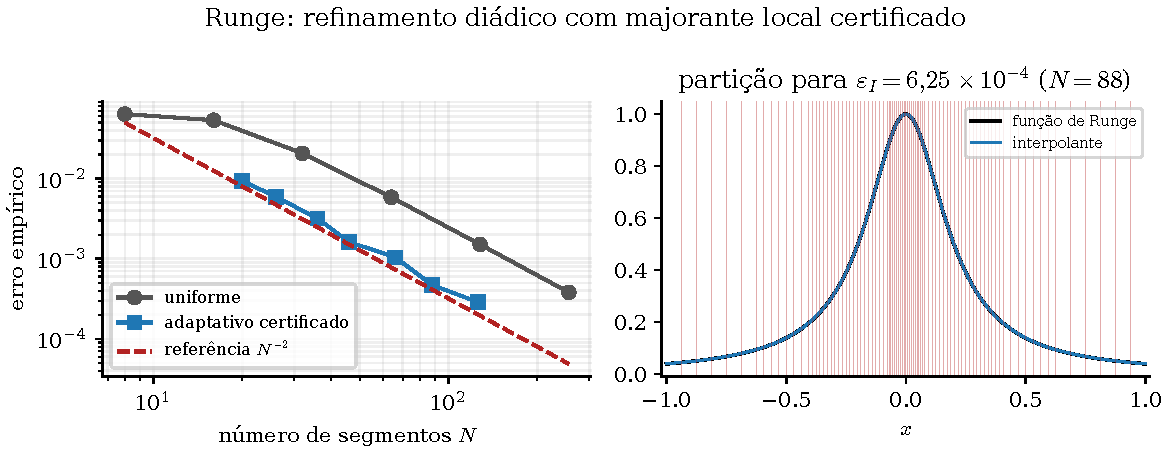
\includegraphics[width=.94\linewidth]{fig05_adaptativo.pdf}
 \caption{Erro empírico e partição adaptativa. A prova da garantia usa o majorante local, não a curva amostrada.}
 \label{fig:adaptive-pt}
\end{figure}

\subsection{Restrição de curvatura e codebook sem fator logarítmico}

A melhoria de \eqref{eq:code-length} não vem de trocar os átomos nem as grades:
vem de contar o codebook com a restrição de diferença segunda em vez de contar
livremente os vetores da grade. Como a afirmação é sobre uma constante
universal, ela é verificável.

O script avalia quatro sondas determinísticas, cada uma reescalada pelo fator
$\min\{R/\|f\|_\infty,\,M/\|f''\|_\infty\}$ para que pertença de fato a
$\mathcal F_{R,M}$ com $R=1$ e $M=8$: a quadrática que satura as duas
restrições simultaneamente, dois harmônicos e a função de Runge reescalada.
Sem esse reescalamento a sonda de Runge teria $\|f''\|_\infty=200$ e ficaria
fora da bola, tornando o teste vazio. Para cada tolerância, verifica-se que
$\varepsilon/2<\delta\le\varepsilon$, que $Mh^2\le4\varepsilon$, que o erro
nodal não excede $\delta/2$, que valores adjacentes são distintos, que cada
peça é um átomo de inclinação racional não nula e que a distorção fica dentro
de $\varepsilon$.

\begin{table}[t]
\centering
\caption{Sucessores admissíveis por nó e comprimento do índice global reescalado.}
\label{tab:codebook-pt}
\small
\begin{tabular}{rrrrrr}
\toprule
$\varepsilon$ & $N$ & sucessores & distorção & $L_\varepsilon^{\mathrm{global}}\sqrt{\varepsilon}$ & antigo $\cdot\sqrt{\varepsilon}$\\
\midrule
$6{,}250\,10^{-2}$ & 8   & 9 & $3{,}90\,10^{-2}$ & $10{,}68$ & $13{,}50$\\
$1{,}562\,10^{-2}$ & 16  & 9 & $9{,}68\,10^{-3}$ & $10{,}34$ & $17{,}00$\\
$3{,}906\,10^{-3}$ & 32  & 9 & $2{,}26\,10^{-3}$ & $10{,}00$ & $20{,}62$\\
$9{,}766\,10^{-4}$ & 64  & 9 & $6{,}98\,10^{-4}$ & $9{,}74$  & $24{,}38$\\
$2{,}441\,10^{-4}$ & 128 & 9 & $1{,}62\,10^{-4}$ & $9{,}56$  & $28{,}22$\\
\bottomrule
\end{tabular}
\end{table}

A \cref{tab:codebook-pt} mostra o essencial. O número de sucessores
admissíveis por nó, dados os dois valores anteriores, é $9$ em todas as
tolerâncias --- abaixo da constante $K=25$ usada na demonstração, que é
portanto conservadora e não ajustada aos dados. As duas últimas colunas são o
diagnóstico do fator logarítmico: o comprimento do índice global da cota atual,
multiplicado por $\sqrt{\varepsilon}$, permanece limitado e até decresce
levemente, enquanto a contagem termo a termo de cada nó cresce
como $\log(1/\varepsilon)$ na mesma normalização. É exatamente a diferença
entre $O(\varepsilon^{-1/2})$ e $O(\varepsilon^{-1/2}\log(1/\varepsilon))$.

\subsection{Contagem de átomos e otimalidade minimax do endereço}

A \cref{tab:enderecos-pt} confronta a contagem exata $|\Library_H|$ com as cotas do
\cref{lem:atom-count} e compara, no pior caso sobre $\Library_H$, o endereço
aritmético $n$ do gerador $\Gamma$ com o endereço $n^\sharp$ da enumeração por
altura da \cref{def:sharp}. A coluna final registra a cota inferior universal,
quanto ao endereçamento sob o calibre fixado, do
\cref{thm:address-lower}. Os expoentes empíricos, obtidos por regressão de
$\log_2(\cdot)$ contra $\log_2H$ nas últimas linhas, aproximam $6$ para
$|\Library_H|$ e $n^\sharp$ e $8$ para $n$, como previsto.

\begin{table}[t]
\centering
\caption{Contagem de átomos por altura e comprimento de endereço no pior caso.}
\label{tab:enderecos-pt}
\small
\begin{tabular}{rrrrr}
\toprule
$H$ & $|\Library_H|$ & $|\Library_H|/(18H^6)$ & $\max n$ ($\Gamma$) & $\max n^\sharp=$ cota inf.\\
\midrule
2 & 252 & 0.2188 & 3231 & 251\\
3 & 3150 & 0.2401 & 87127 & 3149\\
4 & 14168 & 0.1922 & 519638 & 14167\\
6 & 142692 & 0.1699 & 9515572 & 142691\\
8 & 897840 & 0.1903 & 113062957 & 897839\\
12 & 9192456 & 0.1710 & 2233224112 & 9192455\\
16 & 50315232 & 0.1666 & 20668188575 & 50315231\\
24 & 582320976 & 0.1693 & 534070940833 & 582320975\\
32 & 3378271680 & 0.1748 & 5622328883731 & 3378271679\\
48 & 36947682720 & 0.1678 & 131374552971847 & 36947682719\\
64 & 206341325696 & 0.1668 & 1289353431661883 & 206341325695\\
\bottomrule
\end{tabular}

\end{table}

A \cref{fig:enderecos-pt} torna visível a diferença entre os expoentes do
gerador aritmético e da enumeração por cascas, sempre para o calibre
\eqref{eq:atom-height}.

\begin{figure}[t]
 \centering
 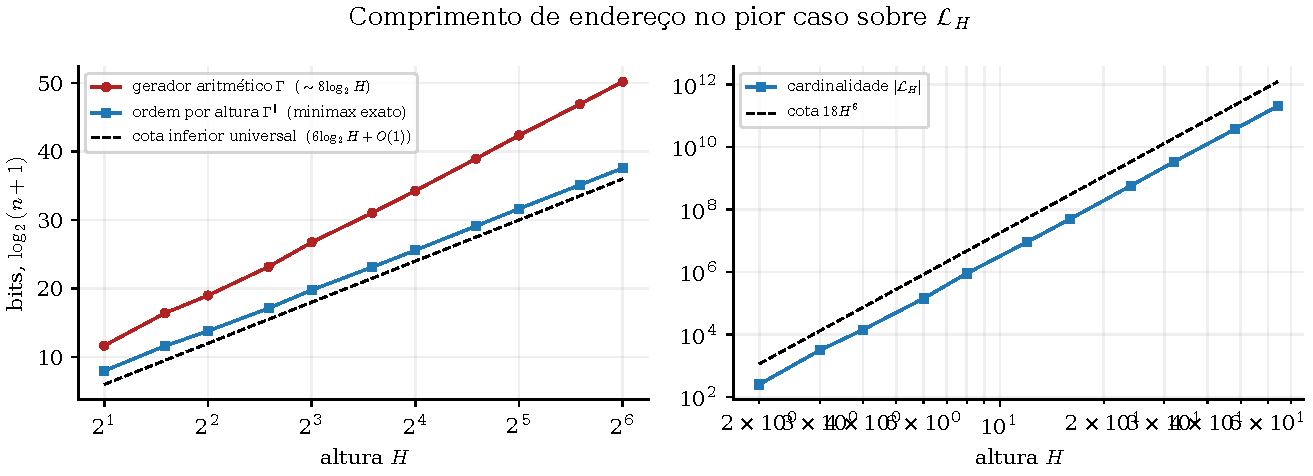
\includegraphics[width=.92\linewidth]{fig06_enderecos.pdf}
 \caption{Comprimento de endereço no pior caso sobre $\Library_H$. A enumeração
 por altura $\Gamma^\sharp$ acompanha a cota inferior relativa a $\Library_H$ com uma folga
 limitada; o gerador aritmético $\Gamma$ paga um fator constante $4/3$ no
 expoente em troca de inversa em forma fechada.}
 \label{fig:enderecos-pt}
\end{figure}

Foi ainda verificada, para $0\le n^\sharp<20{,}000$, a bijetividade de
$\Gamma^\sharp$ nos dois sentidos e a coincidência dos conjuntos
$\Gamma(\{0,\ldots,N\})$ e $\Gamma^\sharp(\{0,\ldots,N'\})$ quando restritos a
uma mesma casca de altura.
